%%==================================================================%%
%% Author : Tejedo Gonz�lez, Daniel                                 %%
%%          S�nchez Barreiro, Pablo                                 %%
%% Version: 1.0, 10/12/2012                                         %%                   %%                                                                  %%
%% Memoria del Proyecto Fin de Carrera                              %%
%% semantica, archivo ra�z                                       %%
%%==================================================================%%

\chapterheader{Sem�ntica del lenguaje}{Implementaci�n de la Sem�ntica, Integraci�n y Despliegue}
\label{chap:semantica}

Este cap�tulo describe la �ltima parte del proceso de desarrollo de nuestro lenguaje: la creaci�n de una sem�ntica que permita la evaluaci�n de las expresiones. Tras las implementaci�n de dicha sem�ntica, se procedi� a la integraci�n del editor creado en el entorno de desarrollo Eclipse, y a su posterior empaquetamiento y despliegue.

\chaptertoc

\section{Introducci�n}
\label{sec:sem:intro}

\todo{Escribe una intro}

\section{Implementaci�n de la sem�ntica del lenguaje}
\label{sec:sem:sem}
%%==================================================================%%
%% Author : Tejedo Gonz�lez, Daniel                                 %%
%%          S�nchez Barreiro, Pablo                                 %%
%% Version: 1.0, 10/12/2012                                         %%                   %%                                                                  %%
%% Memoria del Proyecto Fin de Carrera                              %%
%% semantica, semantica                                      %%
%%==================================================================%%

Implementar la sem�ntica del lenguaje es el �ltimo paso (sin contar las pruebas) para dar por concluido el desarrollo de nuestro editor. La sem�ntica es la que permite que las acciones que se definen en las l�neas de c�digo escritas en el editor sean ejecutadas, luego es una parte bastante importante de todo el proceso.

En el apartado anterior indicamos que el bot�n de Validate era el que, adem�s de cargar la configuraci�n pertinente, iniciaba la validaci�n de las restricciones definidas. Por lo tanto, el inicio de la implementaci�n de la sem�ntica estar� contenido en el marco del manejador del bot�n Validate. 

Desde este manejador cargamos todas las restricciones definidas, e iniciamos el proceso de validaci�n evaluando cada restricci�n una a una. Usaremos el resultado obtenido para constuir un cuadro de di�logo en el que mostraremos el resultado de validar cada una de las restricciones definidas en la configuraci�n previamente seleccionada. 

Para realizar la validaci�n se utiliza el m�todo "evaluate" de la clase Operand. Este m�todo recibe la configuraci�n sobre la que hay que realizar la evaluaci�n, y una caracter�stica que se usar� como contexto. Al estar en la clase abstracta Operand se puede observar que es heredado a su vez por todas las posibles operaciones que pueden expresarse, de modo que cada operaci�n pueda redefinir el m�todo evaluate de acuerdo con la funcionalidad que ha de implementar. 

Por ejemplo, el m�todo evaluate de la clase Plus simplemente retornar� el valor num�rico de la suma de su primer operando y su segundo operando. Teniendo en cuenta de que sus operandos a su vez pueden ser operaciones, la funci�n ha de retonar en realidad el valor de la evaluaci�n del primero de sus operandos sumado al valor de la evaluaci�n del segundo de sus operandos.

De este modo llegar� un momento en que haya que evaluar directamente objetos de clase SimpleFeature, MultipleFeature o Number, que ser�n las hojas del �rbol resultante de parsear la restricci�n. Evaluar un n�mero simplemente consiste en retornar su valor, y evaluar una caracter�stica consiste en comprobar si est� seleccionada (en caso de ser simple) o mirar en cu�ntas ocasiones ha sido seleccionada (en caso de que sea m�ltiple).

As� pues, inicar la tarea de validaci�n en el manejador requiere acceder a la operaci�n m�s significativa de la restricci�n, ya que la clase Constraint no contiene un m�todo evaluate. Conviene recordar que en el metamodelo hab�amos indicado que una restricci�n solo se relaciona con una operaci�n, y las dem�s las consigue mediante las relaciones de sus operandos. Gracias a eso podemos concluir que evaluar la restricci�n es lo mismo que evaluar su operaci�n booleana m�s significativa, a la que se accede directamente desde esa relaci�n, que nos facilita mucho la tarea en este punto.

En general, la implementaci�n del m�todo "evaluate" para la mayor�a de las operaciones es trivial y no conlleva m�s de un par de l�neas de c�digo (como el caso de la suma anteriormente definido). No obstante, algunas operaciones son algo m�s complicadas y requieren algo m�s de reflexi�n. Hablamos de las operaciones que requieren un contexto. Hay que tener en cuenta que, tal como ha sido explicado en cap�tulos anteriores, las operaciones con contexto solo miran una parte muy concreta de la configuraci�n, e implementar fue complicado ya que las evaluaciones se van encadenando y ese contexto puede modificar el comportamiento de otras operaciones.

Para solucionar este problema se a�adi� el par�metro "context", que simplemente es una Feature que indica a partir de qu� punto en la configuraci�n hay que tener en cuenta la evaluaci�n. De este modo tenemos que modificar la implementaci�n de la evaluaci�n de SimpleFeature y MultipleFeature para tener en cuenta esto, y contar para el resultado de la evaluaci�n �nicamente las caracter�sticas que sean hijas de la Feature que se pasa como par�metro.

Una vez se ha concluido de implementar el m�todo evaluate en todas las operaciones y se lanza el proceso desde el manejador del bot�n "Validate" se puede dar por finalizada la fase relativa a la sem�ntica.

\section{Pruebas}
\label{sec:sem:pruebas}

\todo{Escribir algo sobre las pruebas de la sem�ntica}

\section{Integraci�n con Eclipse}
\label{sec:sem:int}
%%==================================================================%%
%% Author : Tejedo Gonz�lez, Daniel                                 %%
%%          S�nchez Barreiro, Pablo                                 %%
%% Version: 1.0, 10/12/2012                                         %%                   %%                                                                  %%
%% Memoria del Proyecto Fin de Carrera                              %%
%% semantica, interfaz                                       %%
%%==================================================================%%

EMF y EMFText proporcionan una interfaz por defecto para la creaci�n de editores y su posterior uso. Se incluyen algunos aspectos como coloreado de palabras clave y detecci�n instant�nea de errores de sintaxis. Es por eso que ya cont�bamos con gran parte del trabajo hecho, y esta ha sido una de las razones por las que EMFText pareci� m�s conveniente en su momento.

La interfaz del editor desarrollado es parte de la herramienta Eclipse y no puede ejecutarse fuera de su entorno. No tendr�a sentido hacerlo de otro modo, ya que no solo necesitamos las diversas funciones que EMF y EMFText nos proporcionan, sino que la propia herramienta Hydra es tambi�n un plug-in de Eclipse. La figura \ref{figeditor} muestra la interfaz del editor en funcionamiento.

\begin{figure}[t]
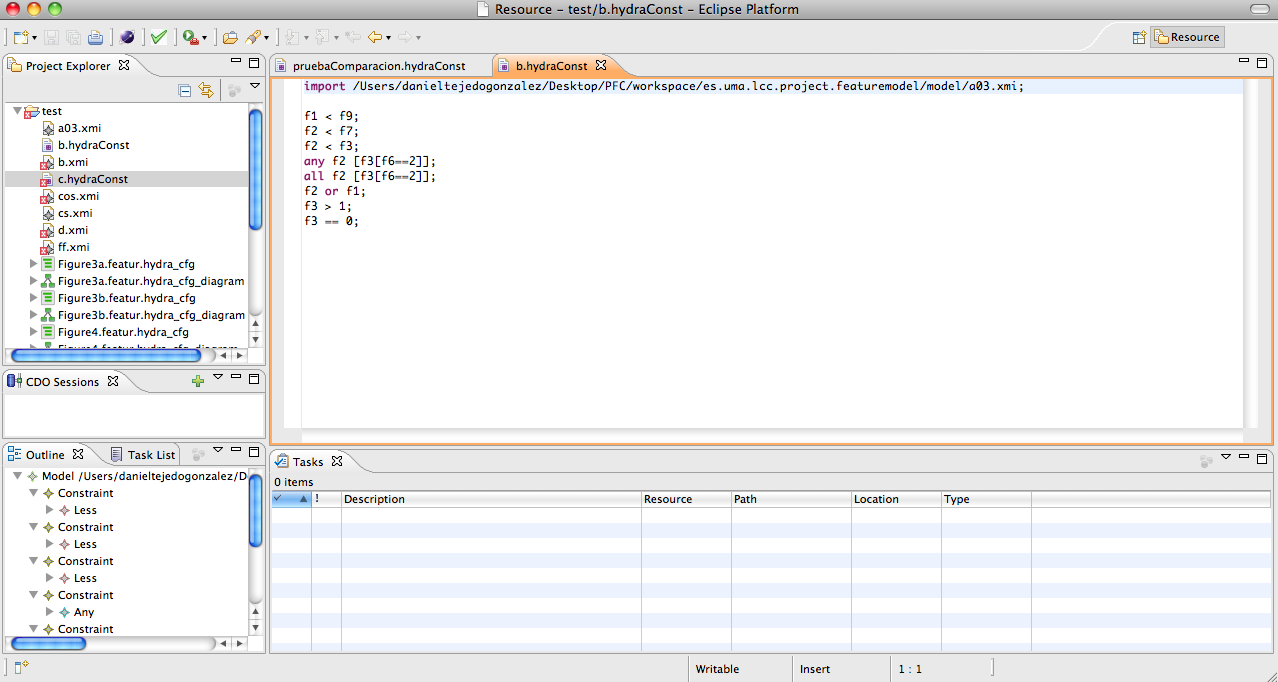
\includegraphics[scale=0.34]{semantica/editor.jpg}
\caption{Captura de pantalla del editor en funcionamiento}
\label{figeditor}
\end{figure} 

Las caracter�sticas del editor creado por defecto por EMF no son suficientes para satisfacer toda la funcionalidad que debe llevar a cabo, por lo que ha sido necesaria una ligera modificaci�n para poder cumplir con los objetivos de nuestra aplicaci�n. Para poder implementar la sem�ntica es necesario que nuestro editor cargue previamente dos modelos: el modelo de caracter�sticas (lo cual ya ha sido implementado) y una configuraci�n de ese modelo, que es sobre el que se validar�n las restricciones que definamos.

Para permitir que se pueda cargar esa configuraci�n hemos a�adido un bot�n llamado "Validate" que abre una ventana de carga en la que se pide al usuario escoger un fichero de extensi�n .xmi exclusivamente. Una vez cargado, el manejador del bot�n ejecutar� la validaci�n y mostrar� el resultado de la misma en un cuadro de di�logo. Pero esto es tarea de la sem�ntica y ser� explicado en el apartado siguiente. 

\begin{figure}[t]
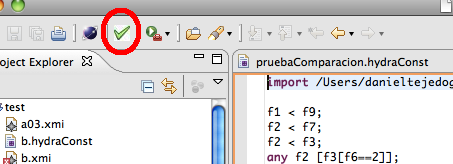
\includegraphics[scale=0.74]{semantica/boton.jpg}
\caption{Bot�n que ejecutar� la validaci�n de las restricciones}
\label{figboton}
\end{figure} 

Dado que nuestra aplicaci�n no es sino un plug-in de Eclipse, a�adir el bot�n ha requerido informarse de la Arquitectura de Plug-ins de Eclipse. Sin entrar en demasiados detalles, el proceso consiste en a�adir lo que se conoce como "punto de extensi�n" al plug-in previo. Un punto de extensi�n sirve para dotar a un plug-in de la funcionalidad de otros plug-ins e incorporarla a ellos. En este caso nuestro punto de extensi�n corresponde a uno proporcionado por la propia arquitectura, cuya utilidad es precisamente la de a�adir botones al men� de herramientas de nuestra aplicaci�n.


\section{Empaquetamiento y Despliegue}
\label{sec:sem:despliegue}
% %%==================================================================%%
%% Author : Tejedo Gonz�lez, Daniel                                 %%
%%          S�nchez Barreiro, Pablo                                 %%
%% Version: 1.0, 10/12/2012                                         %%                   
%% Version: 2.0, 11/03/2013                                         %%                   
%%                                                                  %%
%% Memoria del Proyecto Fin de Carrera                              %%
%% semantica, despliegue                                              %%
%%==================================================================%%

Una vez que se ha implementado la aplicaci�n completamente, el �ltimo paso para finalizar este proyecto es exportarla para que pueda ser utilizada en otros computadores.

Para llevar a cabo esta tarea se ha optado por la creaci�n de un \emph{update site}, que permite instalar la aplicaci�n desde la opci�n \emph{Install New Software} del propio men� de Eclipse. Consideramos que esta era la opci�n m�s c�moda para distribuir nuestra aplicaci�n. El archivo \emph{updateSite.zip} del CD adjunto contiene los ficheros necesarios para llevar a cabo la instalaci�n de nuestro editor.

Adem�s, hemos creado un peque�o manual de usuario que explica de manera r�pida y con muchas im�genes como empezar a utilizar nuestra aplicaci�n. Tambi�n hemos grabado un videotutorial que muestra la aplicaci�n en funcionamiento. Tanto el manual como el v�deo est�n disponibles en el CD adjunto, bajo el nombre de \emph{manual.pdf} y \emph{video.mp4}.

\todo{Escribir algosobre el empaquetamiento y despliegue}

\section{Sumario}
\label{sec:sem:sumario}
% %%==================================================================%%
%% Author : Tejedo Gonz�lez, Daniel                                 %%
%%          S�nchez Barreiro, Pablo                                 %%
%% Version: 1.0, 25/11/2012                                         %%                   
%%                                                                  %%
%% Memoria del Proyecto Fin de Carrera                              %%
%% Sintaxis abstracta, sumario                          %%
%%==================================================================%%

Durante el presente cap�tulo se ha descrito el proceso de definici�n de la sintaxis abstracta de nuestro lenguaje. Este proceso abarca subtareas como la captura de requisitos del lenguaje, la creaci�n de un metamodelo que permita la creaci�n de sintaxis concretas apropiadas, la validaci�n de restricciones externas a ese metamodelo, y las pruebas que corroboren que todos los elementos creados funcionan correctamente. En el siguiente cap�tulo profundizaremos acerca del dise�o de la gram�tica para nuestro lenguaje, as� como de las herramientas utilizadas para implementar esa gram�tica.

\todo{Escribir un sumario}

